\documentclass[sigconf,nonacm,screen]{acmart}

\renewcommand{\sectionautorefname}{Section}
\renewcommand{\subsectionautorefname}{Section}
\renewcommand{\subsubsectionautorefname}{Section}

\usepackage{amsmath}
\usepackage{booktabs}
\usepackage{graphicx}
\usepackage{microtype}
\usepackage{tabularx}

\graphicspath{{figures/}}
\setlength{\emergencystretch}{2em}

\newcommand{\writeestimatedcharactercount}[1]{%
  \immediate\write18{expr `texcount -1 -sum -merge #1.tex` + `texcount -1 -sum -merge -char #1.tex` - 1 > chars.txt}%
}

\AtBeginDocument{\providecommand\BibTeX{{Bib\TeX}}}

\setcopyright{CC}
\setcctype{by-sa}

\begin{document}

\title[Vibe Shuffle]{Vibe Shuffle: Next-Song Selection from Relative Valence--Arousal Trajectories}

\author{Markus Baumann}
\authornote{Corresponding author.}
\affiliation{%
  \institution{Ludwig-Maximilians-Universit\"at M\"unchen}
  \city{Munich}
  \country{Germany}}
\email{markus.baumann@campus.lmu.de}

\author{Felix Hajuj}
\affiliation{%
  \institution{Ludwig-Maximilians-Universit\"at M\"unchen}
  \city{Munich}
  \country{Germany}}
\email{felix.hajuj@campus.lmu.de}

\author{Miriam Janner}
\affiliation{%
  \institution{Ludwig-Maximilians-Universit\"at M\"unchen}
  \city{Munich}
  \country{Germany}}
\email{M.Janner@campus.lmu.de}

\begin{abstract}
Music recommenders learn what listeners like in general, but the song that fits
depends on the moment. Vibe Shuffle asks whether facial and cardiac changes
measured relative to personal references, together with recent camera movement,
can make next-song selection more context-sensitive. At the start of a session
the system initializes personal reference values for facial and cardiac signals. The facial reference then
adapts slowly to longer visible changes, whereas the cardiac reference remains
fixed. Later facial and cardiac observations are expressed as deviations from
the active references, while movement and nodding are summarized over a recent
camera window. The resulting observations are mapped to a valence--arousal plane
without assigning the listener an emotion label. Observations collected during a track form a
short trajectory whose mean identifies a catalog region, and the nearest
unplayed song in that region is selected. An exploratory within-session
crossover compared Vibe Shuffle with Random selection from the same catalog.
Mood-fit ratings were higher on average under Vibe Shuffle while general liking
differed little on average, but the confidence intervals for both differences
included zero, so no recommendation benefit is established. The contribution is
an inspectable method that turns within-session multimodal observations into a single
song-selection decision, together with a blueprint for the study needed to test
it.
\end{abstract}


\begin{CCSXML}
<ccs2012>
  <concept>
    <concept_id>10003120.10003121.10003128</concept_id>
    <concept_desc>Human-centered computing~Human computer interaction (HCI)</concept_desc>
    <concept_significance>500</concept_significance>
  </concept>
  <concept>
    <concept_id>10002951.10003317.10003347.10003350</concept_id>
    <concept_desc>Information systems~Recommender systems</concept_desc>
    <concept_significance>300</concept_significance>
  </concept>
</ccs2012>
\end{CCSXML}
\ccsdesc[500]{Human-centered computing~Human computer interaction (HCI)}
\ccsdesc[300]{Information systems~Recommender systems}

\keywords{affective computing, music recommendation, relative affect,
valence and arousal, heart-rate variability, facial cues, baseline-relative adaptation}

\maketitle

\section{Motivation}

Music choice is contextual. A track that suits exercise may be unwelcome during
a quiet break. People use music to regulate mood and activation
~\cite{juslin2008,schaefer2013}. Most recommender systems prioritize durable
signals such as listening history, favorite artists, similar users, and item
features. Those signals characterize usual preference and capture momentary
fit only indirectly, a known challenge in contextual music recommendation
~\cite{kaminskas2012,schedl2018}. A listener may like a song in general without
wanting it next.

Explicit mood selection can address that gap, but it also interrupts an
otherwise continuous experience. Automatic adaptation offers another route.
Its observations, however, are uncertain. Facial behavior depends on pose,
lighting, culture, context, and deliberate expression
~\cite{barrett2019,aviezer2012,kuppens2017}. Cardiac timing varies with
respiration, posture, movement, fitness, medication, and sensor quality
~\cite{shaffer2017,laborde2017,quigley2024}. Neither channel directly identifies
emotion.

\emph{Vibe Shuffle} uses these uncertain observations only as within-listener
changes that may guide the next song. During setup, the listener
provides short personal camera and cardiac references. Later observations are
expressed as changes from those references. The horizontal axis represents
relative Valence evidence; the vertical axis represents relative Arousal
evidence. Each point falls into a Tense, Energetic, Melancholic, or Calm
recommendation region. These names identify catalog regions, not the
listener's emotional state.

The catalog uses song Valence and Energy coordinates. Vibe Shuffle averages
the recent trajectory, retains unplayed tracks in its region, and selects the
nearest eligible track. Random draws from the same remaining catalog without
the trajectory. The adaptive chain is explicit: personal references, relative
observations, trajectory, region, and nearest available song.

The study compares this policy with Random selection from the same fixed
catalog. Its primary outcome is participant-rated mood fit, analyzed through
the paired difference and the uncertainty around it. Liking is a secondary
measure of general song preference. The comparison rests on three reproducible
elements:
\begin{itemize}
  \item Personal reference periods center camera and cardiac observations
  before the relative Valence and Arousal coordinates are calculated.
  \item Event-driven observations form a trajectory whose mean identifies a
  catalog region and whose distance ranking yields the nearest unplayed track.
  \item The exploratory crossover estimates mood-fit and liking differences
  under matched catalog, exposure, and rating procedures.
\end{itemize}

Mood-fit estimates favored Vibe Shuffle, whereas liking barely changed; both
intervals crossed zero. A service-level evaluation would require validated
sensor mappings, complete trial records, preregistration, and a dynamic catalog.

\begin{figure*}[t]
  \centering
  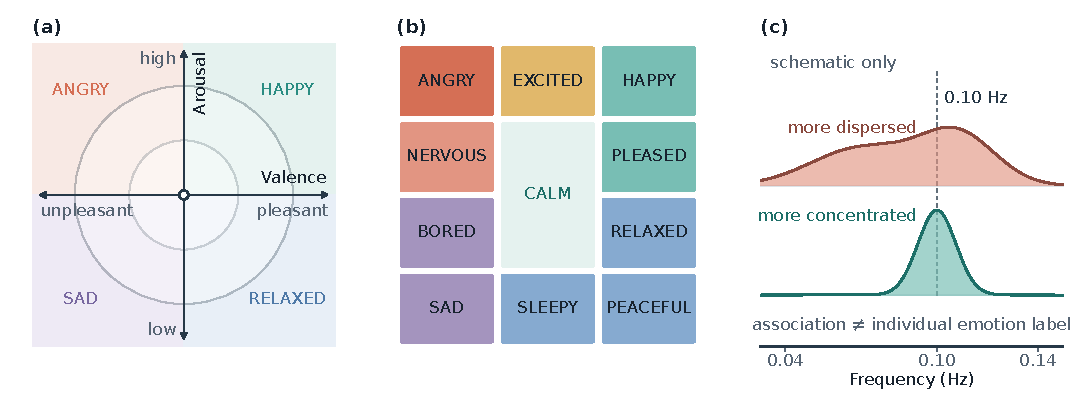
\includegraphics[width=\textwidth]{fig1_affect_space.pdf}
  \caption{Panels (a)--(b) are original redrawings adapted from Helmholz et
  al.~\cite{helmholz2019}, who
  operationalized Russell's circumplex~\cite{russell1980} and Thayer's
  mood--arousal model~\cite{thayer1991}. Panel (c) is an original schematic
  adapted from the group-level frequency distinction reported by Balaji et
  al.~\cite{balaji2025}; it contains no empirical observations.}
  \Description{Three square conceptual panels show a continuous
  valence-arousal plane, a categorical affect vocabulary, and a
  coherence-frequency schematic.}
  \label{fig:affect-space}
\end{figure*}

\section{Background}

\subsection{A relative valence--arousal coordinate}

The circumplex model represents affect along two continuous dimensions:
\emph{valence}, from unpleasant to pleasant, and \emph{arousal}, from low to
high activation~\cite{russell1980,posner2005}. Thayer's account of energetic and
tense arousal offers a complementary vocabulary for changes in activation and
mood~\cite{thayer1991}. These models are useful here as a compact interaction
space, not as a complete account of emotion. Both dimensional and discrete
models appear in music-emotion research, with results sensitive to model and
annotations~\cite{eerola2013}.

Figure~\ref{fig:affect-space} is an independently drawn conceptual synthesis:
it places the continuous and categorical affect vocabularies beside the
strictly group-level HRV-frequency context that motivates an exploratory
diagnostic signal.

\begin{figure*}[t]
  \centering
  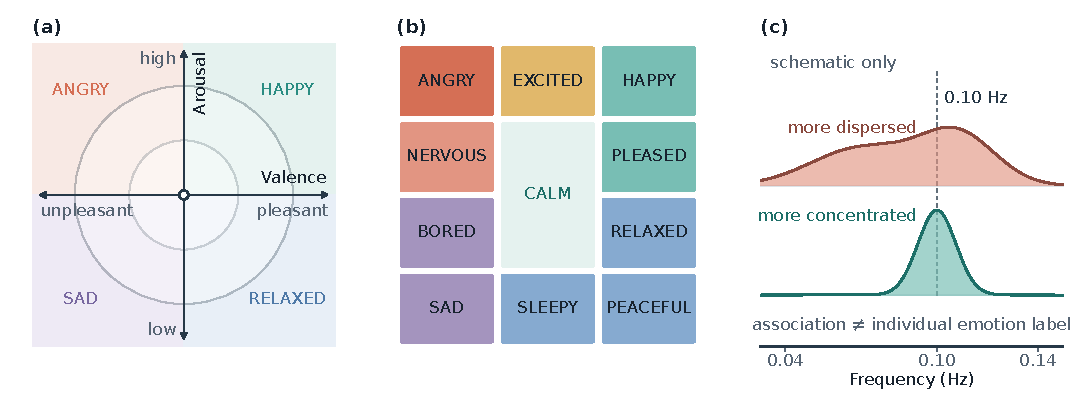
\includegraphics[width=\textwidth]{fig1_affect_space.pdf}
  \caption{\textbf{Conceptual foundations.} Panels (a)--(b) are adapted and
  independently redrawn from Helmholz et al.~\cite{helmholz2019}, Figure~1,
  which operationalizes Russell's circumplex~\cite{russell1980} and Thayer's
  mood--arousal model~\cite{thayer1991}; no source pixels are reused. Panel (c)
  is an original, data-free schematic of the group-level frequency distinction
  discussed by Balaji et al.~\cite{balaji2025}; no curves, observations, or
  source artwork are reproduced or adapted. Illustrations only---not Vibe
  measurements or classifiers.}
  \Description{Three square conceptual panels show a continuous
  valence-arousal plane, a categorical affect vocabulary, and two synthetic
  coherence-frequency profiles explicitly marked as schematic rather than
  data.}
  \label{fig:affect-space}
\end{figure*}

Vibe Shuffle borrows only the two-axis coordinate structure. It does not output
the emotion words shown in Figure~\ref{fig:affect-space} or treat them as
ground-truth labels. The coherence profiles in panel (c) are likewise not the
prototype's diagnostic signal.

Vibe Shuffle places the listener at a point $(V,A)$ in this space and divides
the plane into four quadrants. Crucially, the point describes change relative
to that listener's own reference measurements. The center is the personal
baseline; evidence of more positive facial display moves the point right, while
evidence of greater cardiac activation moves it upward. The system therefore
asks a deliberately narrow question---which direction did the observed signals
move?---rather than attempting to name or recover the listener's full emotional
state. This distinction matters because facial movements are not unique
fingerprints of specific emotions and vary with person and
context~\cite{barrett2019}. Facial judgments can also shift with body context,
and Valence--Arousal relations vary across people and
cultures~\cite{aviezer2012,kuppens2017}.

\subsection{Connecting listener state to music}

Music can be placed in a parallel two-dimensional space. Song \emph{Valence}
describes conveyed positivity, whereas \emph{Energy} describes perceived
intensity and activity. Prior emotion-oriented music interfaces have used these
attributes as musical counterparts to affective valence and
arousal~\cite{helmholz2019}. Vibe Shuffle adopts that practical bridge: listener
Valence is compared with song Valence, and listener Arousal is compared with
song Energy. The alignment is an engineering assumption, not a claim that
musical Energy and physiological Arousal are the same construct.
Music-emotion recognition also uses continuous coordinates, but its annotations
remain subjective~\cite{yang2012}.

The shared plane makes the selection rule easy to inspect. High and low values
on each axis produce four broad regions, and the listener's relative position
determines the target region. Within that region, distance in the continuous
plane distinguishes closer from more distant songs. The quadrants simplify
communication; the underlying coordinate preserves degree and direction.

\subsection{Heart-rate variability as relative evidence}

Heart-rate variability (HRV) describes variation between successive heart
beats. The root mean square of successive differences (RMSSD) is a widely used
time-domain summary of short-term RR-interval variation~\cite{shaffer2017}.
Heart rate and RMSSD depend on respiration, movement, posture, fitness,
medication, sensor quality, and other factors; neither measure identifies a
particular emotion on its own. Good-practice guidance therefore emphasizes
standardized conditions, artifact review, matched durations, and respiration
assessment~\cite{laborde2017}.

Vibe Shuffle consequently uses cardiac measurements only as
baseline-relative evidence for the arousal axis. A heart rate above the
listener's reference and an RMSSD below that reference contribute upward
evidence; changes in the opposite direction lower it. The mapping is transparent
and testable, but remains a prototype heuristic rather
than a clinical or psychological measurement.

\subsection{Related work}

Prior music systems connect listener information with song coordinates in
several ways. \emph{Feel the Moosic} lets the listener choose a position in a
simplified affect space and requests tracks from corresponding Spotify
Valence--Energy ranges~\cite{helmholz2019}. Janssen et al.\ learned
listener-specific relations between music and physiological response and used
them to steer an affective music player toward a goal~\cite{janssen2012}.
Ayata et al.\ estimated Valence and Arousal from wearable
galvanic-skin-response and photoplethysmography measurements~\cite{ayata2018},
while Tran et al.\ matched a facial estimate with nearby tracks in Spotify
feature space~\cite{tran2023}. These systems establish several routes from
explicit or inferred context to music.

Two issues remain. First, classification accuracy does not establish that a
recommended track improves the listening experience. Second, the path from
sensor observation to selection can hide consequential assumptions.
Explanations may support transparency, trust, effectiveness, or
decision-making~\cite{nunes2017}, while user experience also depends on effort,
privacy, and context~\cite{knijnenburg2012}. A reviewable policy should expose
what was observed, how it was summarized, and why one song became eligible.

\subsection{Research gap, questions, and contributions}

Among the systems reviewed here, few expose a baseline-relative path from
multimodal observations to a reviewable next-song decision. It also remains
unclear whether that policy changes listener judgments when catalog, exposure,
and rating procedure are held constant. Vibe Shuffle addresses this gap with a
personal reference, an event-driven listening trajectory, a fixed
region-and-distance rule, and a Random comparator drawn from the same frozen
catalog.

\paragraph{RQ1.}
How can within-listener changes in facial and cardiac observations be
transformed into an inspectable next-song decision without assigning absolute
emotion labels?

\paragraph{RQ2.}
How does Vibe Shuffle compare with Random song selection in participants'
ratings of mood fit and liking?

The paper makes three concrete contributions. First, it defines a
baseline-relative formulation of multimodal music adaptation. Second, it
specifies the path from personal references and listening trajectories to an
eligible-song decision. Third, it reports a matched exploratory comparison
that quantifies the direction and uncertainty of mood-fit and liking
differences. These contributions define a testable policy and its current
evidence boundary.

In the exploratory comparison, mood-fit ratings were 0.56 points higher under
Vibe Shuffle on average, but the confidence interval crossed zero. Liking
differed by 0.09 points and was similarly uncertain. These estimates motivate a
better instrumented test of the policy; they do not show that the system
improves listening.

\section{From Relative Signals to the Next Song}
\label{sec:method}

\subsection{Design principle}

Vibe Shuffle is a client-only React/Vite application. A camera, an optional
Bluetooth Heart Rate Service device, and Spotify playback meet inside one
browser session. There is no study database or recommendation server. The
design keeps adaptation between songs rather than changing playback
continuously: the system listens to the latest window, summarizes it, and then
chooses the next track. This makes the decision legible and prevents every
short-lived fluctuation from becoming a command.

Figure~\ref{fig:trajectory} shows the complete idea. Two personal references
anchor the incoming signals. Confirmed playback produces a path rather than a
single instantaneous label. The path is averaged, mapped to a region, and used
to select a nearby song. A participant then rates the track, closing the
interaction loop.

\begin{figure*}[t]
  \centering
  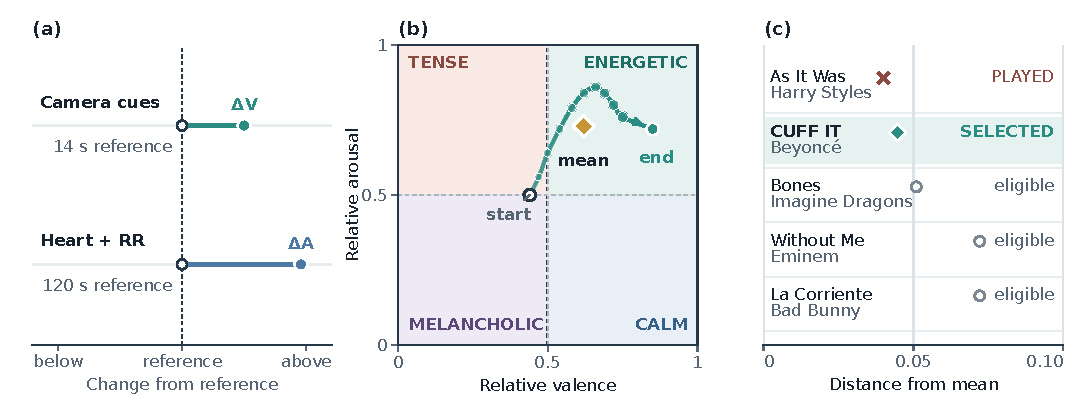
\includegraphics[width=\textwidth]{fig2_relative_trajectory.pdf}
  \caption{\textbf{Relative sensing, trajectory, and selection in Vibe
  Shuffle.} (a) Camera and cardiac inputs are expressed as signed changes from
  personal references. (b) A curved Valence--Arousal trajectory is summarized
  by its arithmetic mean (gold diamond); points grow and darken from the open
  start marker to the filled endpoint. (c) Within the matching region,
  \emph{As It Was} is nearest but
  excluded as played (cross), so \emph{CUFF IT} becomes the selected eligible
  track (filled diamond); open circles are alternatives.
  The relative changes and trajectory are illustrative; catalog candidates,
  distances, and the selection result are repository-derived.
  This is a relative heuristic, not an emotion diagnosis; coherence is logged
  separately and does not affect selection.}
  \Description{Three equal square panels show camera and cardiac changes from
  personal references, a curved illustrative relative valence-arousal
  trajectory with its mean, and a ranked list of five catalog candidates in
  which As It Was is marked played and CUFF IT is selected.}
  \label{fig:trajectory}
\end{figure*}

\subsection{Relative Valence from camera cues}

The browser runs MediaPipe Face Landmarker locally~\cite{mediapipe2019}. It
returns facial blendshape activations such as smile, cheek, brow, eye, jaw,
frown, and mouth movement. Vibe Shuffle combines a selected subset into
transparent positive, negative, and tension-related scores. These labels belong
to Vibe Shuffle's rule layer; MediaPipe itself does not output the project's
emotion-region labels.

A 14-second calibration captures a short facial reference, and a slow running
baseline continues to adapt. Later observations are debiased against this
reference and smoothed across frames. Positive facial evidence moves Valence to
the right; negative or tension-related evidence moves it to the left. If no face
is detected, Valence returns to the neutral center. The current heuristic also
lets visible movement increase positive Valence evidence and upward Arousal
evidence. Movement may instead reflect dancing, repositioning, lighting change,
or camera noise, so this rule is not a validated engagement or affect measure.

\subsection{Relative Arousal from cardiac timing}

The optional wearable provides device-produced beats per minute and, when
available, RR intervals---the elapsed time between successive beats. The
application does not receive a raw electrocardiogram and cannot inspect the
device's peak-detection process. Implausible and abruptly changing RR intervals
are rejected before short-term variability is calculated.

The primary variability feature is the root mean square of successive
differences (RMSSD). A 120-second reference stores the listener's ordinary
median heart rate and typical RMSSD together with robust estimates of their
variation. During listening, higher-than-reference heart rate and
lower-than-reference RMSSD provide upward Arousal evidence. Heart rate receives
the larger influence because RMSSD estimated from a short window is unstable;
when the two disagree, the RMSSD contribution is strongly reduced. At least 20
accepted RR intervals are required before the full estimate is treated as
usable. Controlled resting data show high agreement between 120-second and
longer RMSSD recordings~\cite{munoz2015}; this supports the calibration duration,
not short moving-wearable windows or Arousal validity.

The implementation also exports SDNN and a custom normalized
frequency-domain spectral-peakedness score. The CSV calls this the physiology
coherence field. It is an experimental diagnostic, not the coherence measure
analyzed by Balaji et al., and it does not determine the selected region. Prior
HRV-biofeedback research reports group-level associations between coherence
patterns and end-of-session self-reported emotion
categories~\cite{balaji2025}. That result motivates careful study of cardiac
timing, but it neither validates the prototype's proxy nor shows that a short
personal window can identify an individual's emotion. Vibe Shuffle accordingly
uses baseline-relative activation evidence rather than translating coherence
frequencies into labels.

\subsection{A trajectory rather than a snapshot}

Whenever the fused live coordinate changes during confirmed playback, Vibe
Shuffle appends a point to the current trial buffer. Facial cues primarily
control Valence. Usable cardiac evidence supplies the Arousal base, with visible
movement able to add upward Arousal. If cardiac evidence is unavailable, camera
movement provides an upward-only fallback. If neither channel is usable, the
coordinate returns to $(0.5,0.5)$.

The resulting sequence makes the listener's path visible conceptually:
\[
  \mathcal{T}=\{(V_1,A_1),\ldots,(V_m,A_m)\}.
\]
At rating time, the application uses the arithmetic mean
\[
  (\bar V,\bar A)=\frac{1}{m}\sum_{i=1}^{m}(V_i,A_i)
\]
as the target for the next adaptive choice. The points are event-driven rather
than sampled at a fixed rate, so this is not a time-weighted physiological
average. Sample count and actual listening duration are exported to make that
approximation visible.

\subsection{Four regions and a fixed music space}

Splitting both axes at 0.5 produces four recommendation regions:
Energetic (higher Valence and Arousal), Calm (higher Valence and lower
Arousal), Tense (lower Valence and higher Arousal), and Melancholic (lower on
both axes). The frozen catalog contains 100 Spotify tracks, with 25 tracks in
each corresponding Valence--Energy region. Track coordinates originate from
historical Spotify features in a public dataset~\cite{spotifydataset}. Energy
is a practical catalog-side counterpart of Arousal, not proof that an audio
feature and a physiological construct are identical.

Both Random and Vibe exclude the current and all previously played tracks.
Random ranks the remaining tracks with a session-seeded pseudorandom score.
Vibe first retains available tracks in the target region and then selects the
smallest Euclidean distance:
\[
 s^*=\arg\min_{s\in Q(\bar V,\bar A)}
 \sqrt{(V_s-\bar V)^2+(E_s-\bar A)^2}.
\]
The seed resolves only an exact distance tie. If a region has no remaining
track, the policy falls back to the complete unplayed pool. The export records
the target coordinate, signal source, distance, and region match. It does not
record the random seed, the personal facial-reference values, or individual
trajectory points. The first track is also chosen from the live setup estimate
before the 14-second facial reference is finalized; later choices use the
preceding listening window.

\subsection{Browser implementation and privacy boundary}

Spotify authentication uses Authorization Code with PKCE, and the Web Playback
SDK provides playback for an allowlisted Premium account. Raw camera frames,
facial landmarks, and Bluetooth notifications remain in browser memory. The
locally downloaded CSV contains derived signal summaries, song metadata,
selection fields, ratings, quality flags, pseudonymous identifiers, and
timestamps. It is downloaded automatically at protocol completion and can also
be downloaded manually. It contains no image, landmark set, raw waveform, or
audio. Because it retains only trajectory summaries, it supports review of the
final adaptive target but not replay of every sensing step.

This is a bounded privacy property, not a claim of offline operation. Spotify
authentication and playback, MediaPipe asset delivery, and GitHub Pages create
ordinary external traffic. Exported participant numbers and timestamps are
pseudonymous rather than anonymous and still require appropriate research-data
handling.

\section{Exploratory Crossover Study}
\label{sec:study}

\subsection{Protocol}

The implemented study asks whether the relative adaptive policy feels more
appropriate than Random selection from the same catalog. Every participant
completes one five-track Random block and one five-track Vibe block. Two masked
protocols reverse the order, and odd/even participant numbers suggest the
assignment. Participants see a protocol identifier rather than the condition
name when the operator keeps the participant-facing mode enabled. The same
interface exposes a view toggle and protocol controls, while the experimenter
and exported data can reveal the order. Masking therefore depended on study
administration; it was not technically enforced or double blind. The paired
design is efficient but remains susceptible to practice and carryover, making
reversed order a substantive control~\cite{greenwald1976}.

Each track plays for up to 60 seconds. Participants may select \emph{Rate now};
the actual duration and an early-rating flag are preserved. After each track,
the interface collects a seven-point liking rating, a seven-point mood-fit
rating, and a categorical current-mood report. Mood fit is treated as the
primary outcome in this exploratory report because it directly evaluates the
matching idea. Liking is treated as secondary and helps separate contextual fit
from general song preference.

\subsection{Available evidence}

The supplied analysis report publishes one five-trial condition mean per
participant/session for 15 participants, together with paired tests and
condition-level summaries. These 15 rows are frozen in the repository under
generic analysis IDs. The protocol implies 75 planned ratings per condition and
outcome, but the repository still lacks the underlying trial rows needed to
verify completeness, exclusions, or within-session variation. It also lacks
recruitment records, demographics, and the complete study-administration file.
The present paper therefore treats the participant/session as the inferential
unit and does not claim a fully reproducible human-study archive.

Paired differences are defined as Vibe minus Random. We show the published
participant/session means, report condition means and standard deviations,
paired mean differences with two-sided 95\% confidence intervals, and the
originally supplied paired tests. Because no dated preregistration was
available, all inference is exploratory~\cite{nosek2018}. We foreground paired
effects and confidence intervals rather than a thresholded
$p$-value~\cite{cumming2014}.

\begin{table}[t]
  \caption{Exploratory condition summaries ($N=15$ participants). Confidence
  intervals are two-sided. The reported study tests used one-sided
  Vibe-over-Random alternatives.}
  \label{tab:pilot}
  \centering
  \small
  \begin{tabular}{@{}lccc@{}}
    \toprule
    Outcome & Vibe $M$ (SD) & Random $M$ (SD) & Difference [95\% CI] \\
    \midrule
    Mood fit & 4.71 (0.99) & 4.15 (1.30) & $+0.56$ [$-0.21,1.33$] \\
    Liking   & 4.56 (1.18) & 4.47 (0.77) & $+0.09$ [$-0.52,0.71$] \\
    \bottomrule
  \end{tabular}
\end{table}

\subsection{Results}

Mood fit averaged 4.71 under Vibe and 4.15 under Random
(Table~\ref{tab:pilot}). The paired difference was $+0.56$ rating points, with
a 95\% confidence interval from $-0.21$ to $1.33$ and a standardized paired
effect of $d_z=0.40$. Eight participant/session means were higher under Vibe,
one was tied, and six were lower. The retained directional paired test yielded
$t(14)=1.56$, $p=.070$; the supplied signed-rank sensitivity check yielded
$W^+=74.0$, $p=.088$. The interval includes effects on both sides of zero.

Liking averaged 4.56 under Vibe and 4.47 under Random. The paired difference
was $+0.09$, with a 95\% confidence interval from $-0.52$ to $0.71$ and
$d_z=0.08$. The directional tests yielded $t(14)=0.32$, $p=.375$, and
$W^+=58.5$, $p=.353$. No equivalence margin was specified, so the near-zero
estimate does not establish equivalence.

\begin{table*}[t]
  \caption{Exploratory summaries of 15 participant/session five-trial means.
  Confidence intervals are two-sided; retained tests use one-sided
  Vibe-over-Random alternatives.}
  \label{tab:pilot}
  \centering
  \small
  \begin{tabular}{@{}lcccccc@{}}
    \toprule
    Outcome & Vibe $M$ (SD) & Random $M$ (SD) &
    Difference [95\% CI] & $t(14)$, $p$ & $W^+$, $p$ & $d_z$ \\
    \midrule
    Mood fit & 4.71 (0.99) & 4.15 (1.30) &
    $+0.56$ [$-0.21,1.33$] & 1.56, .070 & 74.0, .088 & 0.40 \\
    Liking & 4.56 (1.18) & 4.47 (0.77) &
    $+0.09$ [$-0.52,0.71$] & 0.32, .375 & 58.5, .353 & 0.08 \\
    \bottomrule
  \end{tabular}
\end{table*}

\begin{figure}[t]
  \centering
  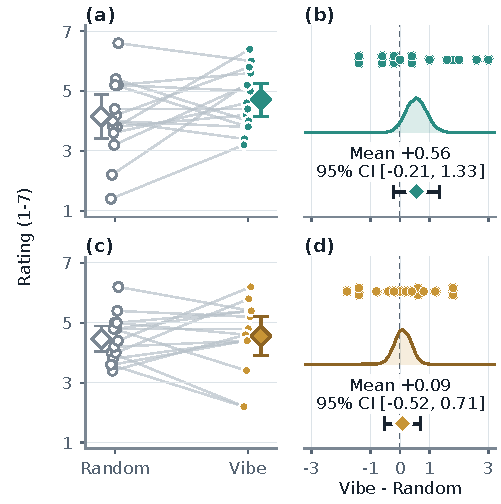
\includegraphics[width=\columnwidth]{fig3_pilot_evidence.pdf}
  \caption{\textbf{Paired participant/session outcomes.} Panels (a)--(b) show
  mood fit; panels (c)--(d) show liking. Left panels connect Random and Vibe
  five-trial means and summarize condition means. Right panels show all paired
  differences, fixed-seed bootstrap mean distributions, and reported paired
  means with $t$-based 95\% CIs. Both paired intervals cross zero.}
  \Description{Four compact panels compare mood fit and liking for 15
  participant-session means. Connected pairs show Random and Vibe ratings;
  estimation panels show paired differences and mean confidence intervals.}
  \label{fig:pilot}
\end{figure}

The pilot does not answer RQ2 decisively. Mood-fit ratings were higher on
average under Vibe Shuffle, whereas liking changed little, but neither estimate
excludes zero or establishes a recommendation benefit.

The paired display also shows heterogeneity that a condition mean would hide.
Several participant/session differences exceed one rating point in either
direction. That variation could reflect music familiarity, starting context,
order, signal availability, or genuine differences in how useful matching is.
The retained means cannot separate these explanations, but they argue against
treating one average response as a universal personalization effect.

\subsection{Reflection and design refinement}

The study and subsequent artifact audit clarify what the project can support.
Personal references provide a local comparison point, but they do not validate
the facial or cardiac mappings. A trajectory makes the decision easier to
inspect, but its arithmetic mean gives more weight to periods with more
coordinate changes. The matched Random condition controls catalog size,
playback path, exposure count, and rating procedure; selected songs can still
differ in artist, genre, language, familiarity, and popularity.

The audit produced concrete refinements to the research specification.
Emotion-detection language was replaced with baseline-relative evidence,
diagnostic coherence was separated from the selection policy, and the decision
record was defined around target, region, distance, signal source, and quality
flags. These changes improve interpretability without strengthening the
historical outcome evidence. No qualitative feedback archive supports claims
of participant-driven redesign.

The signal-processing and selection rules are deterministic JavaScript
modules. Sixty-three tests cover catalog size and balance, export finiteness
and quality flags, facial-rule behavior, RR filtering, baseline-relative
cardiac behavior, and Random/Vibe selection. They validate the present modules,
not sensor accuracy, Spotify playback, the end-to-end study flow, or the code
run during the pilot.

\subsection{Limitations and threats to validity}

Three limitations define the evidence boundary. First, the facial and cardiac
mappings are fixed heuristics rather than independently validated measures.
Movement may alter camera evidence, raise heart rate, and degrade RR quality at
the same time, allowing one behavior to influence both axes. Short HRV windows
and unmeasured respiration further constrain interpretation.

Second, the small exploratory crossover and incomplete archive prevent
trial-level, order, carryover, missing-data, and subgroup analyses. The
retained files contain no recruitment, ethics, hardware, or trial-level
records, so those parts of the study cannot be reconstructed. One-sided tests
should not be treated as confirmatory without preregistration. The first
adaptive choice may precede completed references, sensing is optional, and the
historical summaries do not identify the signal path behind each choice.

Third, the frozen catalog improves experimental control but does not represent
a dynamic streaming service. The conditions share a catalog, not identical
tracks. The system also uses event-weighted rather than time-weighted
aggregation. At the exact no-signal center, current code paths disagree over
whether the boundary belongs to Calm or Energetic. That edge case should be
unified before another study.

\subsection{Next evaluation}

The next evaluation should begin with controlled changes in expression,
lighting, posture, movement, and respiration applied to the frozen mappings.
An instrumented pilot should then require completed references, timing and
missing-data flags, and a complete ten-trial record. Camera-only,
cardiac-only, fused, and Random conditions would identify which evidence path
contributes. Time-weighted and event-weighted trajectory summaries should be
compared directly.

Before a larger crossover, preregister the smallest relevant mood-fit effect,
sample-size justification, exclusions, primary paired analysis, order
analysis, and signal-quality rules~\cite{lakens2022}. A subsequent
dynamic-catalog study should record candidate availability, playback failures,
coverage, catalog revisions, explanations, override behavior, and privacy
expectations. That sequence separates measurement failure from recommendation
failure and tests whether session-aware re-ranking adds value above a
conventional preference model.

\section{Conclusion}

Vibe Shuffle studies baseline-relative music selection from camera and cardiac
observations. It tracks recent movement in Valence--Arousal space, averages the
trajectory, maps that point to one of four regions, and chooses the nearest
eligible song. The trial record identifies the target, region, and distance
used for each recommendation.

In the 15-participant crossover, average mood fit was $0.56$ points higher under
Vibe (95\% CI $[-0.21,1.33]$), and liking was $0.09$ points higher (95\% CI
$[-0.52,0.71]$). The current-mood reports were subjective ratings, and the
research system produced no objective emotion label. The stored target,
signal-source summary, region, and song distance document the final decision;
the trial record omits point-level trajectory samples.

A larger preregistered study should validate the sensor mappings, use
time-weighted fusion, retain complete trial records, and include signal
ablations. If these studies establish a reproducible benefit, a later platform
study could evaluate the policy as a recommendation layer within a
music-streaming service. That evaluation must determine whether
baseline-relative selection improves the perceived fit of what plays next.



\bibliographystyle{ACM-Reference-Format}
\bibliography{bibliography}

\writeestimatedcharactercount{count}

\end{document}
